\documentclass[]{beamer}
% Class options include: notes, notesonly, handout, trans,
%                        hidesubsections, shadesubsections,
%                        inrow, blue, red, grey, brown

\usepackage{beamerthemesplit} 
% Other themes include: beamerthemebars, beamerthemelined, 
%                       beamerthemetree, beamerthemetreebars  
\usepackage[brazil]{babel}
\setbeamertemplate{footline}[frame number] 
\usepackage[utf8]{inputenc}

\beamertemplateballitem %itens mais bonitos, no itemize

\title{Sistemas Multimídia Distribuidos}
\author{}                
\institute{Baseado no cap. 17 do livro do Coulouris\cite{Coulouris:2007}}     
\date{\today}         
%\date{11/08/2011}

\begin{document}

% Creates title page of slide show using above information
\begin{frame}
  \titlepage
\end{frame}

%\section[Roteiro]{}

% Creates table of contents slide incorporating
% all \section and \subsection commands
%\begin{frame}
%  \tableofcontents
%\end{frame}

\begin{frame}[allowframebreaks]
 \frametitle{Panorama}
 \begin{itemize}
   \item Fluxos contínuos de dados em tempo real
   \item Grandes quantidades de áudio, vídeo e outros elementos, respeitando o critério temporal
   \item Elementos de dados distribuídos com atrasos geralmente são eliminados
   \item Especificação: em termos de taxa de passagem de dados (largura de banda),
atraso da distribuição de cada elemento (latência) e taxa de eliminação/perca de pacotes
  \item Latência: especialmente importante em aplicativos interativos
  \item Perca de pacotes é aceitável quando é possível re-sincronizar após o ponto de perda
  \item Alocação de recursos é referida como qualidade de serviços: alocação de processamento,
largura de banda da rede e memória (para buffer)
\end{itemize}
\end{frame}

%\subsection{Introdução}

\section{Introdução}

\begin{frame}[allowframebreaks]
  \frametitle{Introdução}
\begin{itemize}
  \item Fluxos de dados contínuos (streams) baseados no tempo: telefonia pela Internet, 
vídeoconferência, etc
  \item A qualidade geral é ruim; é imprópria para: TV digital/interativa, supervisão com vídeo
  \item Sistemas multimídia são sistemas em tempo real: precisam executar tarefas e apresentar
resultados de acordo com um escalonamento determinado externamente
  \item O grau de sucesso desse fornecimento é o QoS (Quality of Service), usufruída
pelo aplicativo
  \item Diferenças entre os sistemas de tempo real de aviação, processo de fabricação, etc: 
  \item estes possuem volumes de dados pequenos e prazos finais rígidos; o não cumprimento pode ter
consequências desastrosas, por isso superestima-se recursos e trabalha-se com atendimento 
no pior caso
  \item os sistemas multimídia:
  \item operam dentro de um ambiente geral, competindo com recursos e banda de rede com
 outros aplicativos distribuídos
  \item os requisitos são dinâmicos: mais participantes, mais recursos necessários; ou uma 
simulação pode requerer mais processamento
  \item operação de sistemas multimídia em conjunto com outras aplicações: edição de textos, 
conversa de voz separada, mensagens instantâneas, em meio a uma vídeo-conferência
    \item vídeoconferência em desktop
    \item acesso a sequência de vídeo
    \item transmissão de TV e rádio digital
  \end{itemize}
  Recursos para o gerenciamento da qualidade de serviço: largura de banda da rede, ciclos do
processador e capacidade de memória
\end{frame}



\begin{frame}
  \frametitle{Introdução}
   \begin{figure}[hbtp]
  \caption{Sistema Multimídia Distribuído}
  \begin{center}
   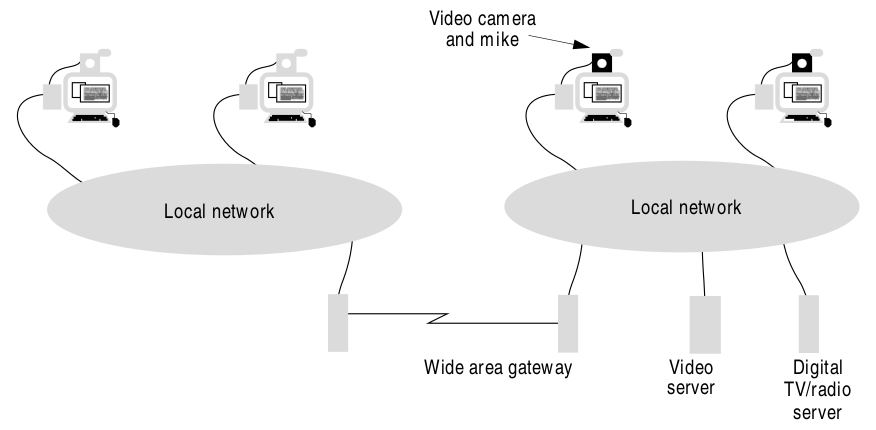
\includegraphics[scale=0.28]{sistema_multimidia_distribuido.png}
  \end{center}
 \end{figure}
\end{frame}

%\begin{frame}
%  \frametitle{Introdução}
%\begin{itemize}
%  \item Sistema distribuído aberto: aplicativos multimídia podem ser iniciados sem organização
%anterior\footnote{O QUE ISSO QUER DIZER EXATAMENTE??} e coexistir na mesma rede
%  \item É necessário haver qualidade do serviço independentemente da qualidade total do sistema
%\end{itemize}
%\end{frame}

\begin{frame}
  \frametitle{Introdução}
Aplicativos multimídia que têm sido implantados:
\begin{itemize}
  \item Multimídia baseada na web: permite acesso aos fluxos de áudio e vídeo na Web; buffers
podem fornecer exibição contínua e suave mas com atraso da origem para o destino (segundos)
  \item Telefone de rede e áudio-conferência: aplicações de natureza interativa com baixos
atrasos de RTT\footnote{round-trip time, tempo de ida e volta}
  \item Vídeo sob demanda: bem sucedidos onde há largura de banda, servidor de vídeo e 
estações, todos dedicados;
alto uso de buffers no destino
\end{itemize}
\end{frame}

\begin{frame}
  \begin{figure}[hbtp]
   \caption{Buffers}
   \begin{center}
    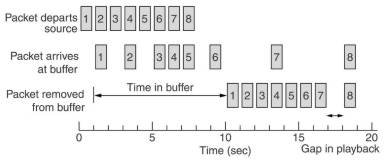
\includegraphics[scale=1.3]{buffer.jpg}
   \end{center}
  \end{figure}
\end{frame}


\begin{frame}
  \frametitle{Introdução}
Aplicativos muito interativos: problemas...
\begin{itemize}
  \item telefonia na Internet - VOIP
  \item vídeoconferência: restrições de largura de banda e latência
  \item ensaio de execução musical distribuída: severas restrições de sincronização
\end{itemize}
\end{frame}

\begin{frame}
  \frametitle{Introdução}
Exigências das aplicações super-interativas
\begin{itemize}
  \item comunicação com baixa latência:
 tela+controle+vídeo+rede+captação < RTT de 100 a 300 ms
  \item estado distribuído síncrono: se um usuário interrompe um vídeo, todos devem 
ver a interrupção no mesmo quadro
  \item sincronismo de mídia: o exemplo da execução musical distribuída; 
Konstantas et al. [1997] aponta até 50ms; fluxos separados de áudio e vídeo devem manter
sincronismo \emph{labial}\footnote{exemplo: sessão de karaokê distribuída}
  \item sincronização externa: aplicações cooperativas diversas devem parecer 
sincronizadas\footnote{Isso é perceptível quando \emph{filmamos a televisão}}
com os fluxos multimídia baseados no tempo (exemplo: animações de computador, dados CAD, 
quadros-negros eletrônicos).   
  \item 
\end{itemize}
\end{frame}

\begin{frame}
  \frametitle{Introdução}
Janela de escassez
\begin{itemize}
  \item Sistemas atuais tem capacidade para manipular dados multimídia
  \item As limitações estão nos recursos necessários, especialmente 
na quantidade e qualidade de fornecimento de fluxos
  \item É necessário alocar e escalonar os recursos
  \item \emph{Antes que a janela de escassez seja alcançada, 
um sistema tem recursos insuficientes para executar as aplicações relevantes}
\end{itemize}
\end{frame}

\begin{frame}
  \frametitle{Introdução}
  \begin{figure}[hbtp]
   \caption{Janela de Escassez}
   \begin{center}
    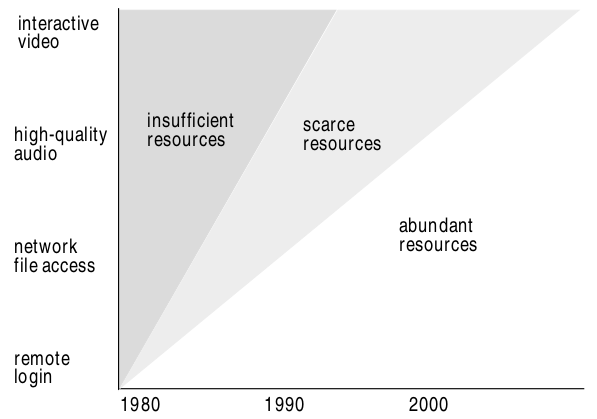
\includegraphics[scale=0.33]{janela_escassez.png}
   \end{center}
  \end{figure}
\end{frame}

\section{Características dos dados multimídia}

\begin{frame}
  \frametitle{Características}
Algumas definições
\begin{itemize}
  \item mídia contínua: sequência de valores discretos que substituem-se uns aos outros
com o passar do tempo; ex: uma imagem é amostrada 25 vezes/seg. para 
dar impressão de movimento com qualidade de TV; um sinal sonoro é amostrado
8000 vezes/seg para transmitir fala com a qualidade de um telefone
  \item fluxos multimídia são baseados no tempo\footnote{ou isocrônicos}: os tempos nos quais
os valores são reproduzidos ou gravados afetam a validade dos dados, definem 
a \emph{semântica} ou conteúdo do fluxo
  
\end{itemize}
\end{frame}

\begin{frame}
  \frametitle{Características}
  \begin{figure}[hbtp]
   \caption{Taxas e Amostras}
   \begin{center}
    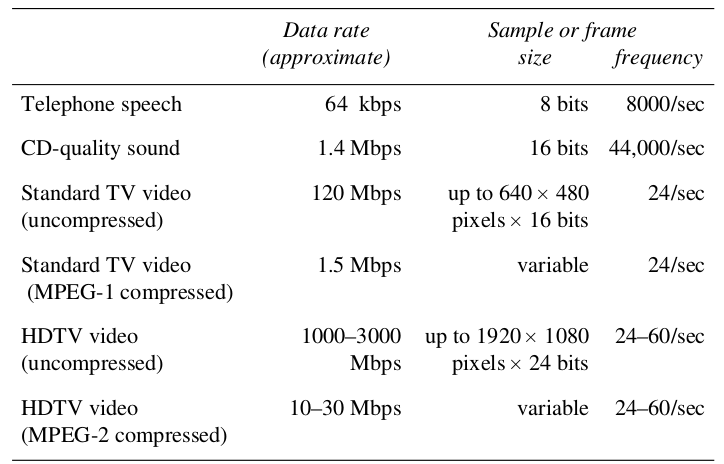
\includegraphics[scale=0.33]{taxas_e_amostras.png}
   \end{center}
  \end{figure}
\end{frame}

\begin{frame}
  \frametitle{Características}
\begin{itemize}
\item dados multimídia são volumosos: precisam de maior desempenho de entrada/saída que os
sistemas convencionais
  \item utiliza-se compactação, embora transformações, como mistura de vídeo, sejam 
difíceis de realizar com fluxos compactados.
  \item compactação pode reduzir requisitos de largura de banda, mas não requisitos de
temporização de dados contínuos
  \item codecs em hardware podem realizar a compactação; codecs em software oferecem
maior flexibilidade
\end{itemize}
\end{frame}

\begin{frame}
  \begin{figure}[hbtp]
   \caption{Pacotes multimídia}
   \begin{center}
    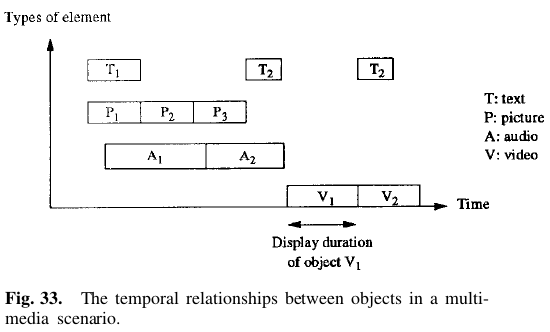
\includegraphics[scale=0.31]{multimedia_packages.png}
   \end{center}
  \end{figure}
\end{frame}

\begin{frame}
  \frametitle{Características}
\begin{itemize}
  \item método MPEG é 
assimétrico\footnote{o codificador é diferente do decodificador}, com algoritmo de compactação complexo e descompactação
simples
  \item isso ajuda em conferências no desktop: compactação feita por codec em hardware, 
descompactação via software
% ????permitindo que o número de participantes na
%vídeoconferência varie sem considerar o número de 
%codecs no computador de cada usuário???? NÃO ENTENDI ESSA FRASE
\end{itemize}
\end{frame}

\section{Gerenciamento de qualidade de serviço}

\begin{frame}
  \frametitle{Gerenciamento da Qualidade de Serviço}
\begin{itemize}
  \item aplicações multimídia executadas em redes de PC's competem por recursos: ciclos 
de processador, barramento, capacidade de buffer)
  \item redes são projetadas pra que mensagens de diferentes origens sejam intercaladas,
permitindo a existência de muitos canais de comunicação virtuais nos mesmos canais físicos
  \item Ethernet: gerencia um meio de transmissão compartilhado na base do melhor esforço
(não-confiável)
  \item enfim: rodízio, tempos aleatórios, etc, podem não satisfazer as necessidades das
aplicações multimídia: distribuição atrasada não tem valor.
\end{itemize}
\end{frame}

\begin{frame}
  \begin{figure}[hbtp]
   \caption{arquitetura abstrata com fluxos de mídia de dados gerados continuamente}
   \begin{center}
    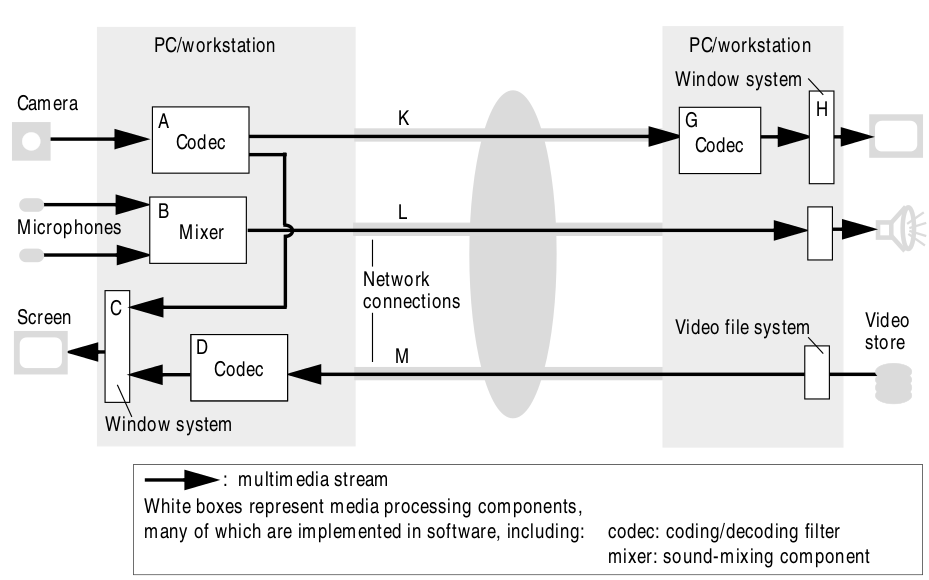
\includegraphics[scale=0.31]{arquitetura_abstrata.png}
   \end{center}
  \end{figure}
\end{frame}

\begin{frame}
  \frametitle{QoS: Negociação}
A aplicação especifica requisitos de qualidade através de 3 parâmetros: 
\begin{itemize}
  \item largura de banda: a taxa na qual os dados fluem pelo fluxo
  \item latência: tempo exigido para um elemento de dados individual se mover
em um fluxo, da origem até o destino; a variação dessa latência é denominada \emph{jitter}
  \item taxa de perda: quadros de vídeo ou amostras de áudio eliminados; até 1\%; 
para aplicações críticas, bem menos!
\end{itemize}
\end{frame}

\begin{frame}

  \begin{figure}[hbtp]
   \caption{requisitos de recurso para a arquitetura abstrata}
   \begin{center}
    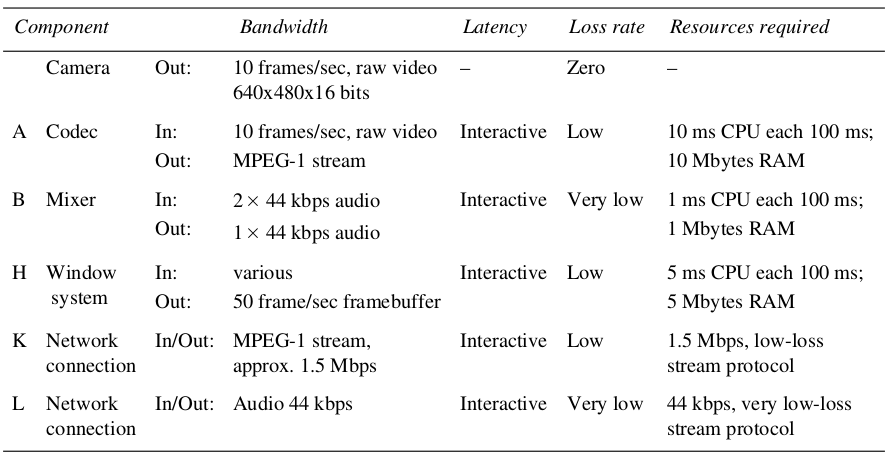
\includegraphics[scale=0.33]{requisitos_recursos.png}
   \end{center}
  \end{figure}
\end{frame}

\begin{frame}
  \begin{figure}[hbtp]
   \caption{Tarefas do negociador de QoS}
   \begin{center}
    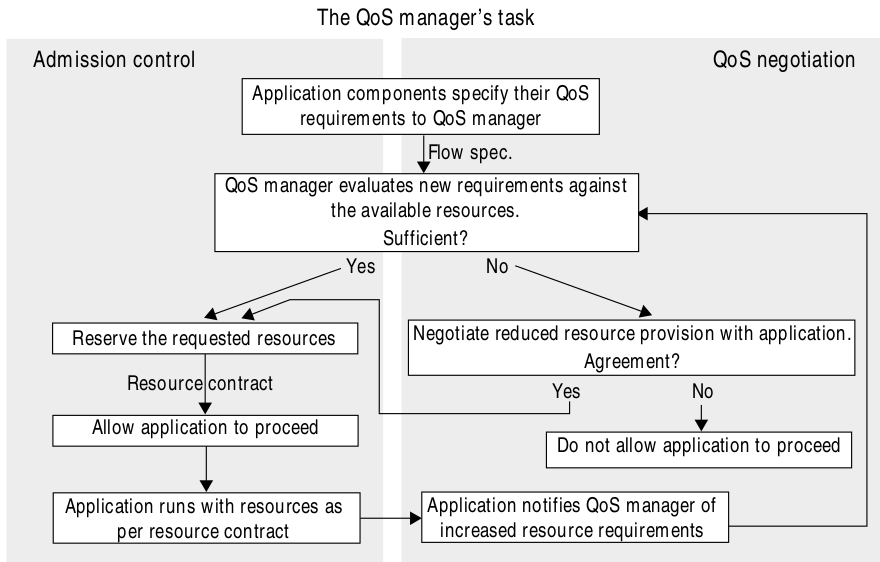
\includegraphics[scale=0.33]{negociador_qos.png}
   \end{center}
  \end{figure}
\end{frame}




%\begin{frame}
%  \begin{figure}[hbtp]
%   \caption{Jitter\cite{site2:2011}}
 %  \begin{center}
 %   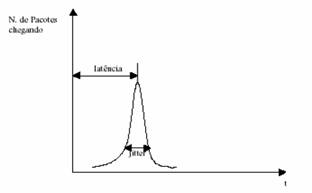
\includegraphics[scale=1.2]{jitter.jpg}
   %\end{center}
  %\end{figure}
%%\end{frame}

%\begin{frame}
   %%\begin{figure}[hbtp]
  %\caption{Jitter}
  %%\begin{center}
%   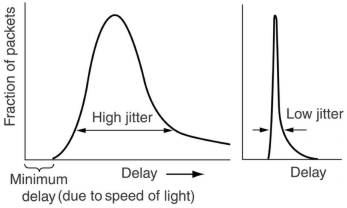
\includegraphics[scale=1.1]{jitter2.jpg}
  %\end{center}
 %%\end{figure}
%\end{frame}

\begin{frame}
   \begin{figure}[hbtp]
  \caption{Jitter\cite{Mingyang:2002}}
  \begin{center}
   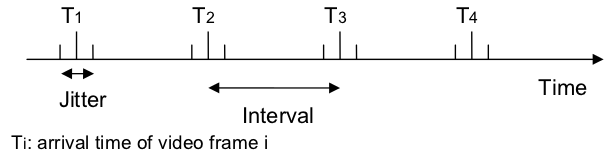
\includegraphics[scale=0.48]{jitter2.png}
  \end{center}
 \end{figure}
\end{frame}

\begin{frame}
   \begin{figure}[hbtp]
  \caption{}
  \begin{center}
   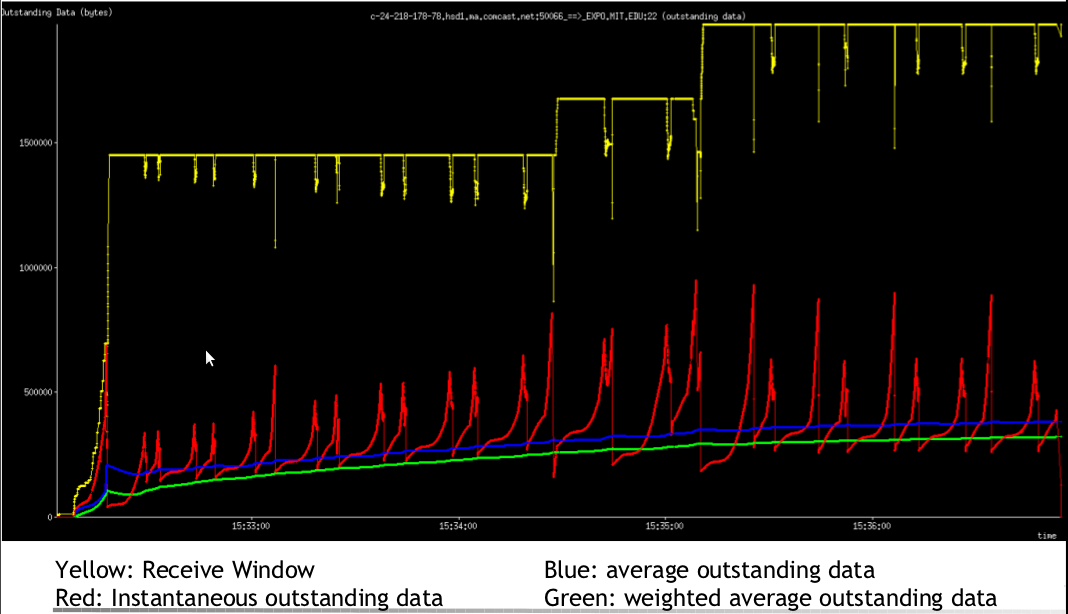
\includegraphics[scale=0.28]{tcp_outstanding_data.png}
  \end{center}
 \end{figure}
\end{frame}

\begin{frame}
   \begin{figure}[hbtp]
  \caption{}
  \begin{center}
   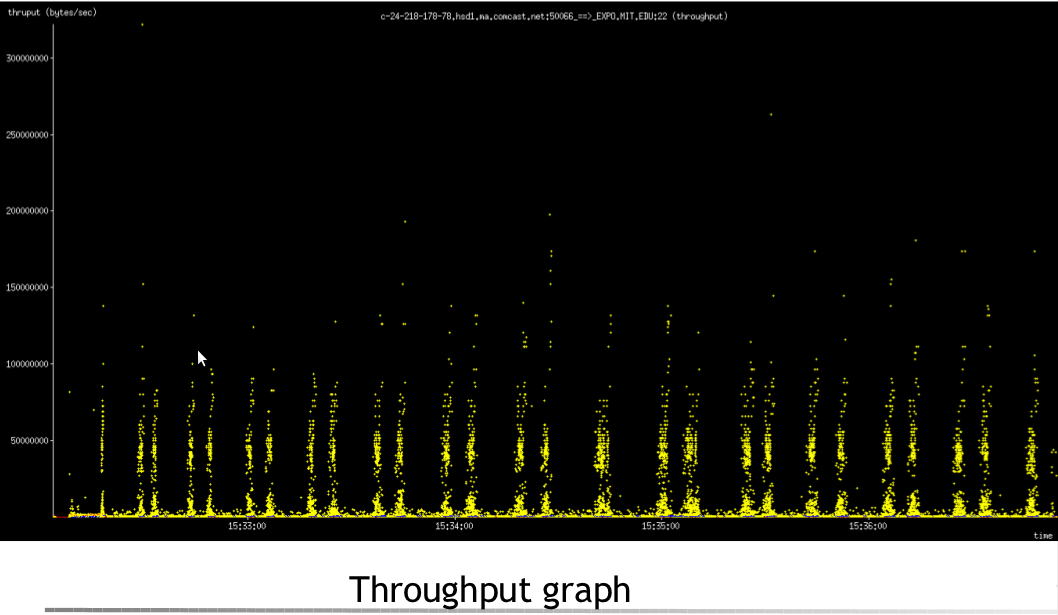
\includegraphics[scale=0.28]{throughput.png}
  \end{center}
 \end{figure}
\end{frame}

\begin{frame}
  \frametitle{QoS: Negociação}
Exemplos de descrição dos parâmetros: 
\begin{itemize}
 \item descrevendo as características de um fluxo: numa aplicação de conferência,
é preciso largura de banda média de 1,5Mbps; atraso máximo
de 150ms para evitar hiatos na palestra; o algoritmo de descompactação
no destino pode produzir imagens aceitáveis com uma perda de 1 quadro em 100
  \item descrevendo capacidade de fluxo: uma rede pode fornecer conexões de largura de banda
de 64kpbs; os algoritmos de enfileiramento garantem atrasos de menos de 10ms; o sistema
de transmissão garante uma taxa de perda menor que 1 em 10e6.
\end{itemize}
\end{frame}

\begin{frame}
  \frametitle{Exemplo de parâmetros: h.264}
 \begin{itemize}
  \item codec/decoder de vídeo
  \item 1080p @ 3.7Mpbs, 720p @ 2.2 Mpbs, 480p @ 1.25 Mpbs :  
  \item perda de pacote aceitável 
até 25\%\footnote{url{http://x264dev.multimedia.cx/archives/249}}
 \end{itemize}
\end{frame}

\begin{frame}
  \frametitle{Exemplo de parâmetros: CELT}
 \begin{itemize}
  \item codec/decoder de áudio
  \item 200 ms aceitavel, 20ms p/ música
  \item atraso de audio < 20ms = 8 metros p/ som no ar
  \item latência: 5ms
  \item bitrate: 32kpbs @ 48kHz stereo
 \end{itemize}
\end{frame}

\begin{frame}
  \frametitle{QoS: Negociação}
Os parâmetros são interdependentes. Exemplos:
\begin{itemize}
  \item taxa de perda depende de estouro do buffer e dados dependentes do tempo
chegando atrasados; logo, quando maior a largura de banda e o atraso, menor será
a taxa de perda
  \item quanto menor a largura de banda, em relação à carga, 
mais mensagens serão armazenadas e mais buffers serão necessários; quanto maior o buffer,
mais provável que mensagens esperem outras que estão na frente para serem atendidas, e
assim, maior será o atraso. 
\end{itemize}
\end{frame}

\begin{frame}[allowframebreaks]
  \frametitle{QoS}
Especificando parâmetros de QoS: largura de banda
\begin{itemize}
  \item  para MPEG, a compactação média está entre 1:50 e 1:100, a depender
do conteúdo; logo, parâmetros de qualidade são 
citados como valores mínimo, médio e máximo.
  \item taxa de rajada 
(\emph{burst}): considere 3 fluxos de 1Mbps: o primeiro 
transfere um único quadro de 1Mbit/s;
o segundo é um fluxo assíncrono de elementos de animação
com largura de banda média de 1Mbps; o terceiro envia amostra de 
som de 100bits a cada microssegundo. 
Os 3 fluxos exigem a mesma largura de banda, porém
seus padrões de tráfego são diferentes. 
O parâmetro de rajada define o número máximo de 
elementos de mídia que podem chegar cedo, 
isto é, antes do que devam chegar, de acordo
com a taxa normal.
 \item Outro exemplo sobre o conceito de rajada é: 
 uma CPU transfere dados via canais ou barramento 
de duas maneiras, byte a byte ou então em blocos de bytes de cada vez; 
é esta modalidade de transferência em blocos é 
chamada de 'modo rajada'.\cite{site1:2011}
\end{itemize}
\end{frame}


\begin{frame}
  \frametitle{QoS}
\begin{itemize}
  \item %Anderson 
%\cite{Anderson:1993} 
Método LBAP (linear-bounded arrival processes): 
%BAIXAR: Meta-scheduling for distributed continuous media, em ACM
define o número máximo de mensagens em um fluxo durante qualquer intervalo t como Rt+B,
onde R é a taxa e B é o tamanho máximo da rajada.
  \item reflete bem dados multimídia: dados multimídia lidos do disco são geralmente 
distribuídos em blocos grandes,
e recebidos das redes em pacotes pequenos; o parâmetro de rajada define a quantidade de
espaço exigida no buffer para evitar perda.
\end{itemize}
\end{frame}

\begin{frame}
  \frametitle{QoS}
Especificando Latência
\begin{itemize}
  \item requisitos do fluxo: um quadro não deve permanecer em buffer, 
em média, por mais do que 1/R,
onde R é a velocidade de taxa de quadros de um fluxo,
 senão ocorrerá acúmulo de trabalho. 
  \item requisitos da aplicação: ex. conferência, atrasos 
de ponta a ponta absolutos de não
mais do que 150ms; reprodução de vídeo, resposta aos comandos
 Pausa e Parar teve ter latência
máxima da ordem de 500ms
  \item jitter\footnote{variação no período entre a
 distribuição de dois quadros subjacentes}: o
uso de buffers resolve, mas há um limite. 
\end{itemize}
\end{frame}

\begin{frame}
  \frametitle{QoS}
Taxa de perda
\begin{itemize}
  \item é o parâmetro mais difícil de especificar; resultam do cálculo de probabilidade 
estouro em buffers e mensagens atrasadas, baseados em pior caso ou distribuição padrão.
  \item taxas de perda dadas para período de tempo infinito são inúteis: qualquer perda
em um tempo curto pode ultrapassar a taxa de longo prazo.
\end{itemize}
\end{frame}

\begin{frame}
  \frametitle{QoS}
Moldagem de tráfego
\begin{itemize}
  \item Termo que descreve o uso de buffers de saída para suavizar o fluxo de dados.
%  \item modelo LBAP\footnote{ANDERSON 1993 VER REFERÊNCIA} de variações de largura de banda 
%exige regular a taxa de rajada dos fluxos multimídia.
  \item Fluxos podem ser regulados pela inserção de um buffer na origem e um método de 
consumo.
\end{itemize}
\end{frame}

\begin{frame}
  \begin{figure}[hbtp]
   \caption{QoS}
   \begin{center}
    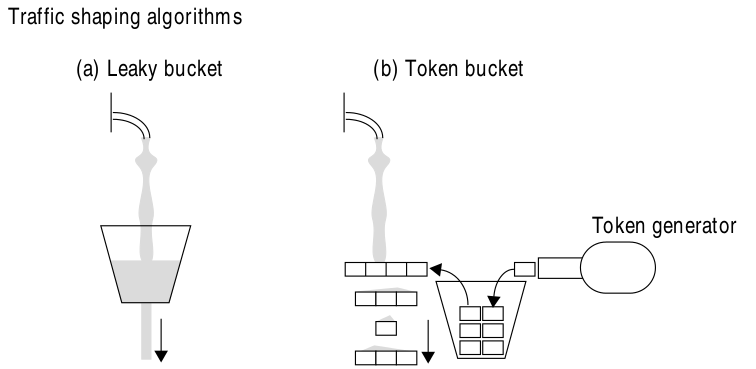
\includegraphics[scale=0.33]{balde_furado.png}
   \end{center}
  \end{figure}
\end{frame}

\begin{frame}
  \begin{figure}[hbtp]
   \caption{QoS}
   \begin{center}
    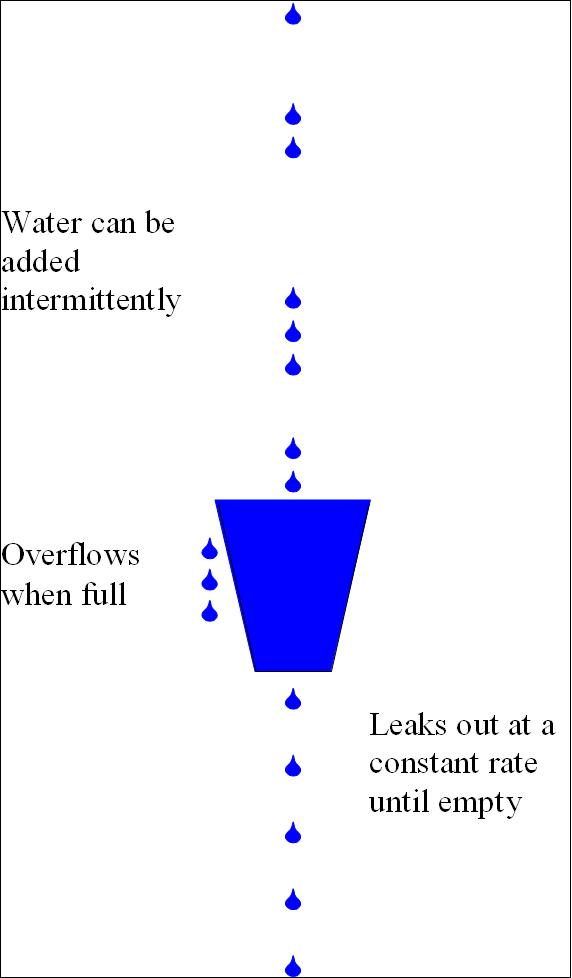
\includegraphics[scale=0.23]{leakybucket.jpg}
   \end{center}
  \end{figure}
\end{frame}

\begin{frame}
  \begin{figure}[hbtp]
   \caption{QoS}
   \begin{center}
    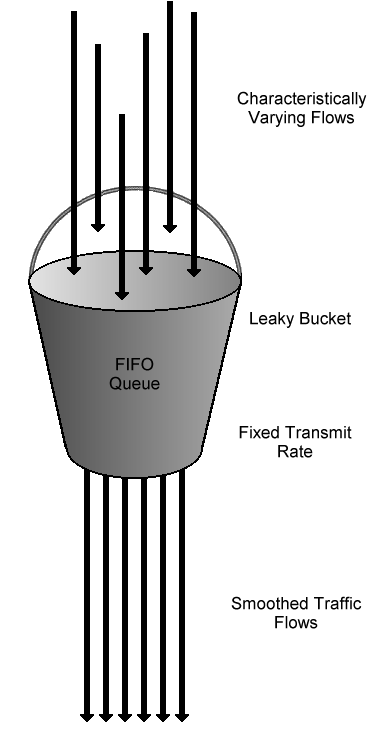
\includegraphics[scale=0.2]{leakybucket2.png}
   \end{center}
  \end{figure}
\end{frame}

%tocketbucket3 e 4.jpg
%http://www.cisco.com/en/US/docs/ios_xr_sw/iosxr_r3.2/qos/configuration/guide/qc32cong.html

%jitter2.jpg, buffer.jpg, tokenbucket3.gif e leakybucket.gif
%http://www.cs.ru.nl/~ths/a3/html/h5/h5.html

%leakybucket.jpg, leakybucket2.jpg
%http://en.wikipedia.org/wiki/Leaky_bucket

\begin{frame}
  \frametitle{QoS - Especificações de fluxo}
 Um conjunto de parâmetros de qualidade de serviço são conhecidos 
como especificação de fluxo; há vários exemplos de especificações de fluxo
e são todos semelhantes, compostos pelos itens:
  \begin{itemize}
   \item unidade de transmissão máxima e taxa de transmissão máxima determinam largura de 
banda máxima exigida pelo fluxo
   \item tamanho do balde com tokens e a taxa determinam a taxa de rajada do fluxo
   \item atraso mínimo que uma aplicação pode observar e o jitter máximo que ela
pode aceitar
   \item número total aceitável de perdas em certo intervalo e número máximo de perdas
consecutivas
  \end{itemize}
\end{frame}

\begin{frame}
  \frametitle{QoS}
  \begin{figure}[hbtp]
   \caption{Agrupamento dos parâmetros, especificao de 
fluxo RFC REC 1363}
   \begin{center}
    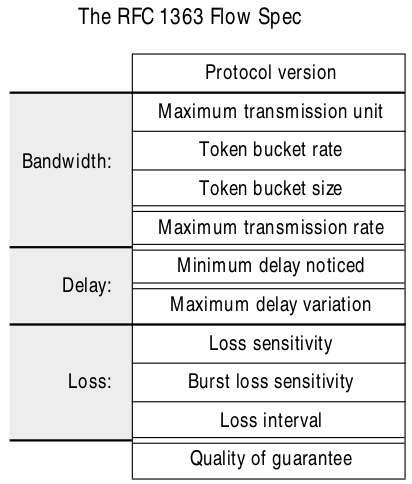
\includegraphics[scale=0.24]{rfc1363.png}
   \end{center}
  \end{figure}

\end{frame}

\begin{frame}
  \frametitle{QoS - procedimentos de negociação}
\begin{itemize}
  \item os gerenciadores de qualidade de serviço estão nos nós
  \item estratégia simples de negociação: envio da especificação de fluxo para o gerenciador
da QoS total; verificação no banco de dados local; encaminhamento para o próximo nó, até
 o destino final; no retorno da mensagem obtem-se a informação sobre a 
viabilidade do fornecimento de serviço
  \item aplicações têm requisitos de qualidade de serviço fixos
  \item é mais apropriado o sistema determinar qual tipo de QoS pode fornecer, e a aplicação
decide se é aceitável
  \item é comum especificar um valor desejado e um pior valor
  \item exemplo: aplicação deseja largura de banda 1,5Mbps, mas pode manipular 1Mbps; o atraso
deve ser 200ms, mas 300ms seria o pior caso aceitável.
\end{itemize}
\end{frame}

\begin{frame}
  \frametitle{QoS - procedimentos de negociação}
\begin{itemize}
  \item fluxo com vários destinos: a negociação bifurca de acordo
com o fluxo de dados; são produzidos valores de pior caso para cada parâmetro da QoS;
exempos: protocolos SRP, ST-II e RCAP.
  \item situações com destinos heterogêneos: negociação iniciada pelo destino: 
RSVP; origens comunicam a existência
dos fluxos; destinos se conectam aos nó mais próximo através do qual o fluxo passa a extrair
dados de lá.
\end{itemize}
\end{frame}

\begin{frame}
  \frametitle{QoS - controle de admissão}
\begin{itemize}
  \item regula o acesso aos recursos para evitar sobrecarga e proteger pedidos que não possam
ser por eles atendidos
  \item baseado em conhecimento geral da capacidade global do sistema e carga gerada
por cada aplicação
  \item recursos com alocador único: simples para controlar a admissão
  \item recursos com pontos de acesso distribuídos: algoritmo 
de controle de admissão distribuído, para tratar concorrências e conflitos.
\end{itemize}
\end{frame}

\begin{frame}
  \frametitle{QoS - reserva de largura de banda}
\begin{itemize}
  \item para fornecer uma QoS garantida: reserva para sua largura de banda máxima
  \item aplicações que se tornam inúteis se houver quedas de qualidade
  \item exemplos: raio X (sintoma aparecer bem no momento de descarte de quadros); 
armazenamento de vídeos (falhas serão visíveis sempre quando reproduzir o vídeo).
  \item cálculo simples: em rede de largura de banda B podem ser admitidos s fluxos
multimídia de largura de banda bs, desde que $\sum_{bs} <= B$
  \item uma rede token ring com 16Mb/s pode suportar até 10 fluxos de vídeo digital de
1,5Mb/s.
\end{itemize}
\end{frame}


\begin{frame}
  \frametitle{QoS - reserva de largura de banda}
\begin{itemize}
  \item alocar largura de banda de CPU exige conhecimento do perfil de execução do processo
aplicativo, que depende do processador usado; não podem ser calculados com precisão.
  \item tempos de execução não são amplamente usados; têm margens de erro grandes e 
portabilidade limitada.
  \item há disperdício quando usa-se reserva baseada nos requisitos máximos.
\end{itemize}
\end{frame}

\begin{frame}
  \frametitle{QoS - multiplexação estática}
\begin{itemize}
  \item suposição: para grande número de fluxos, a largura de banda total
permanece constante
  \item quando um fluxo enviar muitos dados, outro fluxo enviará poucos
  \item isso só ocorrerá em fluxos não-relacionados
  \item experiências mostram que o tráfego em ambientes típicos contradiz essa hipótese:
o tráfego agregado mostra semelhança com os fluxos individuais dos quais é composto
\end{itemize}
\end{frame}

\section{Gerenciamento de recursos}

\begin{frame}
  \frametitle{Gerenciamento de recursos}
  o recurso precisa ter capacidade suficiente (desempenho) e estar disponível
(escalonamento) quando a aplicação precisar
\end{frame}

\begin{frame}
  \frametitle{Ger. de recursos - escalonamento}
\begin{itemize}
  \item processos tem prioridades, determinada por critérios
  \item uso intenso de E/S recebem maior prioridade
  \item em multimídia, prazos finais para distribuição dos dados alteram o escalonamento
  \item exemplo típico: fluxo multimídia é recuperado do disco, enviado pela rede para
uma estação destino, sincronizado com um fluxo proveniente de outra origem e 
exibido: escalonamento de vários recursos
\end{itemize}
\end{frame}

\begin{frame}
  \frametitle{Ger. de recursos - escalonamento}
Escalonamento imparcial (fairness)
\begin{itemize}
  \item fluxos concorrentes pelo mesmo recurso: imparcialidade para evitar que
fluxos mal comportados ocupem largura de banda em demasia
  \item estratégia simples: escalonamento em rodízio em fluxos da mesma classe
  \item trabalhos que realizam esse escalonamento pacote por pacote, e bit por 
bit\footnote{pacotes não podem ser enviados bit a bit, mas dada uma taxa de quadros é possível
calcular, para cada pacote, quando ele será enviado completamente}.
  \item é possível estabelecer que, para certos fluxos, um número maior de bits seja transmitido
por ciclo: enfileiramento imparcial ponderado (priorização no rodízio).
\end{itemize}
\end{frame}

\begin{frame}
  \frametitle{Ger. de recursos - escalonamento}
Escalonamento em tempo real
\begin{itemize}
  \item escalonamento EDF (Earliest-deadline-first): método tradicional que se adapta
bem aos fluxos multimídia contínuos regulares
  \item prazos finais são associados aos itens de trabalho; itens com prazos finais mais
adiantados são processos primeiro.
  \item escalonamento RM (Rate-monotonic): baseado nos elementos que existem por um tempo maior
  \item quanto maior a velocidade dos itens de um fluxo, maior é a prioridade do fluxo
\end{itemize}
\end{frame}

\section{Adaptação de fluxo}

\begin{frame}
 \frametitle{Adaptação de FLuxo}
 \begin{itemize}
   \item quando uma QoS não pode ser garantida, a aplicação precisa de adaptar
   \item forma mais simples: eliminar informações
   \item facilmente realizável em áudio, onde as amostras são independentes, mas notado
imediatamente pelo ouvinte\footnote{Demonstra-se que as pessoas são menos tolerantes a erros
de áudio do que erros de vídeo; assim, em competições pode ser atribuído ao áudio
maior prioridade.\cite{Liao:1997}}
   \item exclusões de quadros em vídeos Motion JPEG são toleráveis: os quadros têm posições livres
   \item MPEG: interpretação de um quadro depende dos valores de quadros adjacentes: omissão
pode amplificar erros
  \end{itemize}
\end{frame}

\begin{frame}
 \frametitle{Motion JPEG x 
MPEG\footnote{\url{http://www.axis.com/products/video/about_networkvideo/compression.htm}}}
  \begin{figure}[hbtp]
  \begin{center}
   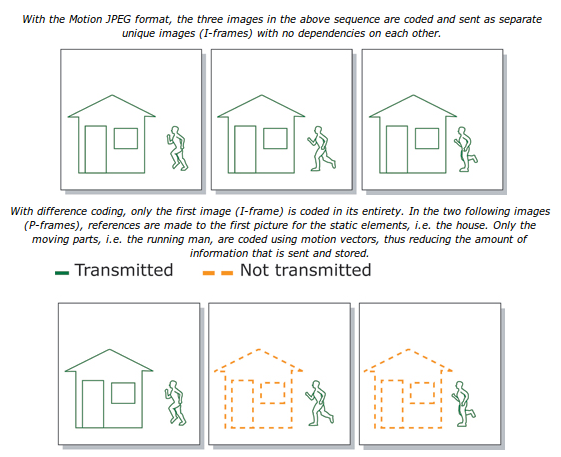
\includegraphics[scale=0.28]{mpeg_x_motionjpeg.png}
  \end{center}
  \end{figure}
\end{frame}

\begin{frame}
 \frametitle{Compressão JPEG}
  \begin{figure}[hbtp]
  \begin{center}
   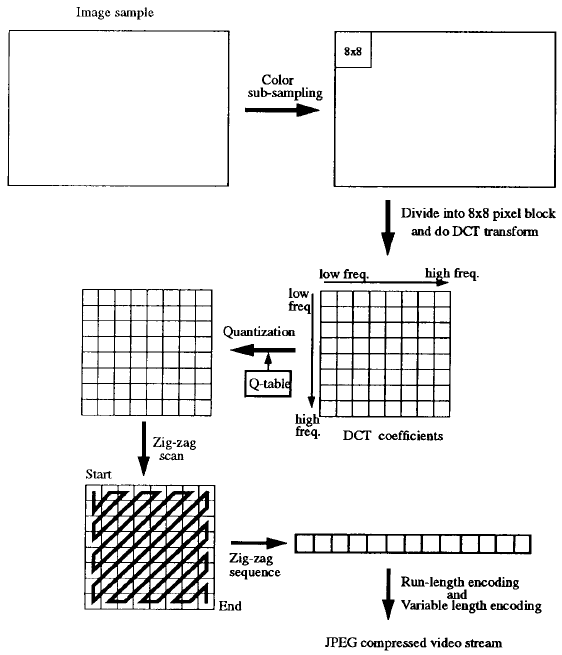
\includegraphics[scale=0.28]{jpeg_compression.png}
  \end{center}
  \end{figure}
\end{frame}



\begin{frame}
 \frametitle{Adaptação de FLuxo}
 \begin{itemize}
   \item largura de banda insuficiente e dados não eliminados: atraso de fluxo aumentará
   \item aceitável em aplicações não-interativas, apesar de possibilitar estouro de buffer
   \item aplicações interativas: se um fluxo estiver atrasado em seu tempo de término designado,
sua taxa de término deverá ser aumentada até que ele esteja novamente no tempo certo: os quadros
 devem aparecer na saída assim que estiverem disponíveis.
  \end{itemize}
\end{frame}

\begin{frame}
 \frametitle{Adaptação de FLuxo: mudanças na escala}
 \begin{itemize}
   \item adaptação realizada apenas no destino em um fluxo: sobrecarga persistirá
   \item adaptar um fluxo para a largura de banda disponível: mudança de escala
   \item operação fundamental: fazer uma nova amostragem do sinal
   \item exemplos: áudio, eliminação de um canal estéreo; mudança de taxa de amostragem
 \end{itemize}
\end{frame}

\begin{frame}
 \frametitle{Adaptação de FLuxo: mudanças na escala}
 \begin{itemize}
   \item vídeo: 
     \begin{itemize}
       \item temporal: diminui o número de quadros transmitidos dentro de um intervalo;
apropriado para quadros individuais independentes
        \item espacial: reduz o número de pixels em cada imagem (diferentes resoluções); 
        \item frequência: modifica o algoritmo de compactação aplicado às imagens
        \item amplitude: reduz intensidades de cores de cada pixel da imagem;
        \item espaço de cores: reduz o número de entradas no espaço de cores; cores para
escala de tons;
     \end{itemize}
     \item Podem ser usadas combinações destas mudanças
  \end{itemize}
\end{frame}

\begin{frame}
 \frametitle{Adaptação de FLuxo: mudanças na escala}
 \begin{itemize}
   \item um monitor controla tempos de chegada de mensagens
   \item mensagens atrasadas indicam gargalos
   \item uma mensagem para \emph{diminuir escala} é enviada, e a largura do fluxo é
reduzida; após algum período de tempo, a origem aumenta novamente a escala
  \end{itemize}
\end{frame}

\begin{frame}
 \frametitle{Adaptação de FLuxo: filtragem}
 \begin{itemize}
   \item mudança de escala modifica o fluxo na origem; nem todos os destinos teriam 
problemas para manipular o fluxo original
   \item a filtragem fornece a melhor QoS possível para cada destino
  \end{itemize}

  \begin{figure}[hbtp]
%    \caption{Filtragem}
   \begin{center}
    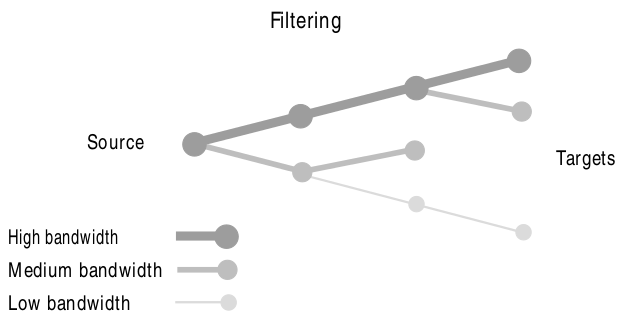
\includegraphics[scale=0.26]{filtering.png}
   \end{center}
  \end{figure}

\end{frame}

\begin{frame}
  \frametitle{Filtragem II \cite{Mingyang:2002}}
  \begin{figure}[hbtp]
  \begin{center}
   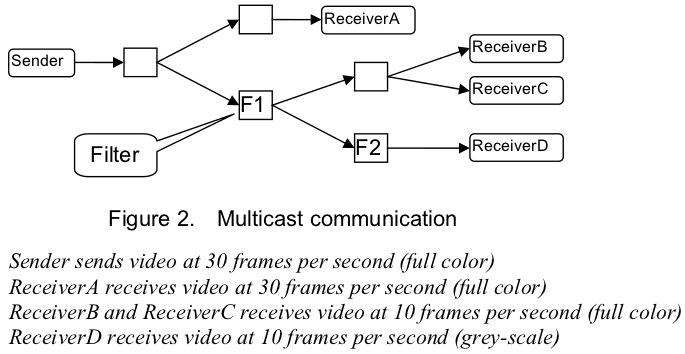
\includegraphics[scale=0.44]{filter_multicast.png}
  \end{center}
 \end{figure}
\end{frame}

\begin{frame}
  \begin{figure}[hbtp]
  \caption{Distribuição em camadas\cite{Moraes:2009}}
  \begin{center}
   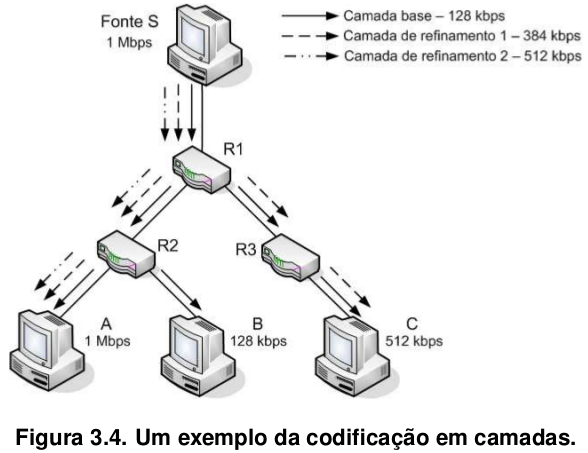
\includegraphics[scale=0.35]{distribuicao_camadas.png}
  \end{center}
  \end{figure}
\end{frame}


\section{Estudo de caso: servidor de arquivos de vídeo Tiger}

\begin{frame}
 \frametitle{Servidor Tiger: objetivos do projeto}
 \begin{itemize}
   \item vídeo sob demanda para grande número de usuários; exemplo: fornecimento de filmes
para clientes pagantes; execução de operações de pausa, retrocesso e avanço rápido; poucos filmes
populares, resultado em várias reproduções concorrentes deslocadas no tempo
   \item QoS: fornecimento com uma velocidade constante, flutuação (jitter) máxima (pequena)
definida pela quantidade de buffers disponíveis nos clientes e taxa de perda mínima
   \item sistema com mudança de escala e distribuído: arquitetura extensível 
(+ computadores) para suportar até 10.000 clientes
   \item hardware de baixo custo: pc's comerciais com unidades de disco padrão
   \item tolerante a falhas: funcionamento sem degradação notável após falha de computadores 
servidores ou discos
  \end{itemize}
\end{frame}

\begin{frame}
 \frametitle{Servidor Tiger: arquitetura}
 todos os componentes são produtos de prateleira;
o controlador é: ponto de contato com os clientes; servidor de hora local; outras
pequenas tarefas\cite{Bolosky:1997}
  \begin{figure}[hbtp]
 % \caption{Arquitetura Tiger\cite{Bolosky:1997}}
  \begin{center}
   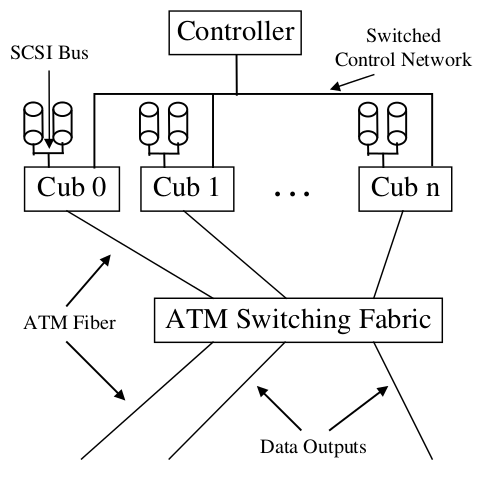
\includegraphics[scale=0.28]{tiger_architecture.png}
  \end{center}
 \end{figure}
\end{frame}

\begin{frame}
 \frametitle{Servidor Tiger: armazenamento}
 \begin{itemize}
   \item filmes são armazenados de forma segmentada (strips) entre todos os discos
   \item a perda de um disco resulta em uma lacuna em cada filme
   \item tratamento: espelhamento de armazenamento e outros descritos a seguir
  \end{itemize}
\end{frame}

\begin{frame}
 \frametitle{Servidor Tiger: segmentação (stripping)}
 \begin{itemize}
   \item filme é dividido em blocos, em torno de 1s, ocupando 0,5 Mb;
   \item blocos que formam um filme (7000, para 2hs) são armazenados em sequência de discos;
um filme pode começar em qualquer disco
   \item ao atingir o disco mais alto, o filme \emph{circula} para o disco 0 e o
processo continua
  \end{itemize}
\end{frame}

\begin{frame}
 \frametitle{Servidor Tiger: espelhamento}
 \begin{itemize}
   \item um bloco é divido em partes, chamadas secundários
   \item quando um cub falhar, a carga cai sobre outros cubs, não sobre um apenas
   \item número de secundários por bloco: fator de desagrupamento d (tipicamente entre 4 e 8)
   \item secundários de um bloco i são armazenados nos cubs i+1 a i+d
   \item desde que existam mais do que d cubs, nenhum dos discos é ligado
no mesmo cubs do disco i
  \end{itemize}
\end{frame}

\begin{frame}
 \frametitle{Servidor Tiger: armazenamento}

  \begin{figure}[hbtp]
 % \caption{Arquitetura Tiger\cite{Bolosky:1997}}
  \begin{center}
   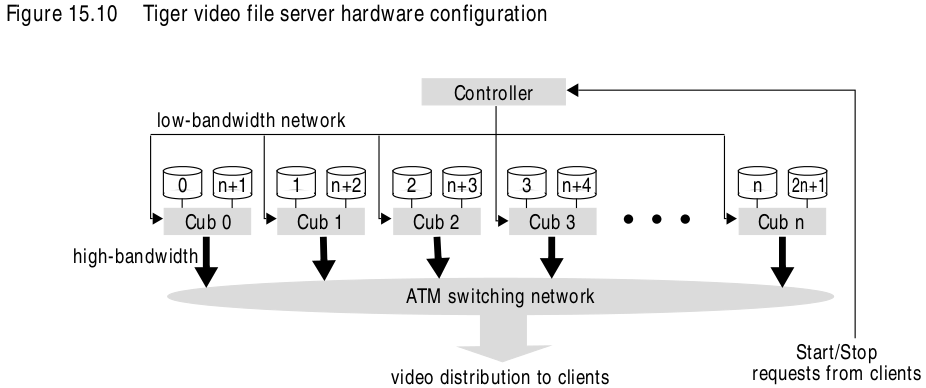
\includegraphics[scale=0.28]{cubs_tiger.png}
  \end{center}
 \end{figure}
\end{frame}

\begin{frame}
 \frametitle{Servidor Tiger: escalonamento distribuído}
 \begin{itemize}
   \item organização por repartições (slots): cada repartição representa o trabalho a ser
feito para reproduzir um bloco de um filme (lê-lo do disco relevante e 
transferí-lo para a rede ATM)
   \item existe uma repartição para cada cliente em potencial receber um 
filme (visualizador); cada
repartição ocupada representa um visualizador recebendo um fluxo de dados de vídeo em tempo
real
  \end{itemize}
\end{frame}

\begin{frame}
 \frametitle{Servidor Tiger: escalonamento distribuído}
O estado do visualizador é representado no escalonamento pelo(a):
 \begin{itemize}
       \item endereço do computador cliente
       \item ID do arquivo sendo reproduzido
       \item posição do visualizador no arquivo (próximo bloco a ser distribuído no fluxo)
       \item número de sequência no visualizador (a partir do qual calcula-se tempo de
distribuição para o próximo bloco)
       \item algumas informações de contabilidade
 \end{itemize}
\end{frame}

\begin{frame}
 \frametitle{Servidor Tiger: tolerância a falhas}
 \begin{itemize}
  \item recuperação de dados das cópias secundárias espelhadas, quando um bloco primário
torna-se indisponível
%    \item 
 \end{itemize}
\end{frame}

\begin{frame}
 \frametitle{Servidor Tiger: suporte de rede}
 \begin{itemize}
  \item blocos de cada filme são passados para a rede ATM pelo cub que o contêm
  \item rede ATM possui QoS para entregar  o bloco ao cliente
  \item cliente apenas verifica o número de sequência do bloco recebido
  \item secundários sendo servidos: os d cubs distribuem na rede (em sequência) e 
o cliente reúne-os e monta-os em seu buffer
 \end{itemize}
\end{frame}

\begin{frame}
 \frametitle{Outras funções}
  \begin{itemize}
   \item implementação inicial: escalonamento e distribuição eram manipulados pelo
controlador
   \item problema: único ponto de falha e gargalo de desempenho em potencial
   \item solução: escalonamento refeito, onde os cubs executam um algoritmo distribuído, 
em tempo não programado, em resposta aos comandos do controlador
   \item alucinação coerente: termo usado para a implementação distribuída de um objeto
compartilhado
   \item nenhum cub tem uma cópia de todo o agendamento, mas age como se houvesse um
estado global coerente
  \end{itemize}
\end{frame}

\begin{frame}
 \frametitle{Servidor Tiger: desempenho e escalabilidade}
 \begin{itemize}
  \item 1994: 5 PC's pentim 133MHz, 48Mb RAM, 3 discos SCSI de 2Gb, 1 controlador ATM,
Windows NT
  \item 68 clientes de filmes, sem falhas, distribuição perfeita
  \item 1 cub danificado (3 discos), perda de dados de 0,02\%
 \end{itemize}
\end{frame}

\section{Referências}

\subsection{Adicionais}

\begin{frame}
 \frametitle{Adicional: aplicações\cite{Maxlow:2003}}
  \begin{itemize}
   \item operações cirúrgicas remotas
   \item controle remoto exploratório de robôs
  \end{itemize}
\end{frame}

\begin{frame}
 \frametitle{Adicional: definições\cite{Maxlow:2003}}
  \begin{itemize}
   \item A estrutura da Internet não é suficiente para fornecer a qualidade, confiabilidade
e interatividade necessária para conteúdo multimídia
   \item Os sistemas multimídia distribuídos adicionam arquiteturas e protocolos
ao topo da Internet (LAN's) para garantir níveis de qualidade
   \item Clientes adicionais não precisam degradar o sistema: eles podem ser recusados se
os recursos são escassos
  \end{itemize}
\end{frame}

%\begin{frame}
% \frametitle{}
% \begin{itemize}
%   \item 
%  \end{itemize}
%\end{frame}



%\begin{frame}
% \frametitle{Questionário, exemplo I}
%  \begin{figure}[hbtp]
%  \begin{center}
%   \includegraphics[scale=0.28]{imagens/questionario_exemplo1.png}
%  \end{center}
% \end{figure}
%\end{frame}


\begin{frame}
 \frametitle{FIM}
   FIM% - Obrigado
\end{frame}



\bibliographystyle{plain}
\bibliography{refs}

\end{document}